% 原书物理页=印刷页69--73；2.6 全节.
\section{根系}\label{sec:lie-2-6}

\begin{definition}\label{def:lie-2-6-1}
设 $V$ 是一个有限维 $\mathbb R$-向量空间. $V$ 中的一个（既约）\newterm{lie-root-system}{根系}{root system}是指如下数据：两个集合 $\Phi\subset V$ 与 $\Phi^{\vee}\subset V^{*}$，并配备一个双射 $\alpha\mapsto\alpha^{\vee}$，使得：
\begin{enumerate}[label=\roman*)]
\item $\Phi$ 有限，在 $\mathbb R$ 上生成 $V$，且 $0\notin\Phi$；
\item 对任意 $\alpha\in\Phi$，$\alpha^{\vee}(\Phi)\subset\mathbb Z$；
\item 对任意 $\alpha\in\Phi$，$\alpha^{\vee}(\alpha)=2$，并且在令 $s_{\alpha}(v):=v-\alpha^{\vee}(v)\alpha$ 时，$s_{\alpha}(\Phi)=\Phi$；
\item 对任意 $\alpha\in\Phi$，$\Phi\cap\mathbb R\alpha=\{\pm\alpha\}$.
\end{enumerate}
$V$ 的维数称为该根系的\newterm{lie-root-system-rank}{秩}{rank}，而 $\alpha^{\vee}$ 称为与根 $\alpha$ 相伴的\newterm{lie-coroot}{对偶根}{coroot}.
\end{definition}

\begin{example*}
设 $\mathfrak g$ 是一个半单 $K$-Lie 代数（$K$ 为特征为零的代数闭域），$\mathfrak h$ 是一个 Cartan 子代数，$\Phi\subset\mathfrak h_{\mathbb Q}^{*}\subset\mathfrak h^{*}$ 是根的集合，而 $\Phi^{\vee}=\{H_{\alpha},\,\alpha\in\Phi\}\subset\mathfrak h_{\mathbb Q}\subset\mathfrak h$. 那么根据前一命题，
\[
(V:=\mathbb R\otimes_{\mathbb Q}\mathfrak h_{\mathbb Q}^{*},\,\Phi,\,\Phi^{\vee},\,\alpha\mapsto\alpha^{\vee}:=H_{\alpha})
\]
是一个根系.
特殊情形：$\mathfrak g=\mathfrak{sl}_{n}(K)$ 且 $\mathfrak h=\{$对角矩阵$\}$. 设 $e_{1},\cdots,e_{n}$ 是 $\mathbb R^{n}$ 的典范基，$e_{1}^{*},\cdots,e_{n}^{*}$ 是它的对偶基. 此时可以把 $(\mathfrak g,\mathfrak h)$ 的根系描述如下：
\[
V=\Bigl\{\textstyle\sum_{i=1}^{n}x_{i}e_{i}\in\mathbb R^{n},\ \sum_{i=1}^{n}x_{i}=0\Bigr\}\subset\mathbb R^{n}
\;\text{与}\;
V^{*}=\Bigl\{\textstyle\sum_{i=1}^{n}x_{i}e_{i}^{*}\in(\mathbb R^{n})^{*},\ \sum_{i}x_{i}=0\Bigr\}\subset(\mathbb R^{n})^{*},
\]
其中的对偶配对由 $\mathbb R^{n}$ 与 $(\mathbb R^{n})^{*}$ 之间的配对诱导，并且
\[
\Phi=\{\alpha_{ij}=(e_{i}-e_{j}),\ 1\leqslant i\neq j\leqslant n\}
\;\text{与}\;
\Phi^{\vee}=\{\alpha_{ij}^{\vee}=(e_{i}^{*}-e_{j}^{*}),\ 1\leqslant i\neq j\leqslant n\},
\]
其中的双射是显然的.
\end{example*}

\begin{numpara}[Weyl 群]\label{np:lie-2-6-2}
注意到上面对定义中 iii) 点引入的 $V$ 的自同态 $s_{\alpha}$ 是以 $\operatorname{Ker}(\alpha^{\vee})$ 为轴、以 $\mathbb R.\alpha$ 为方向的\newterm{lie-reflection}{反射}{reflection}. 换言之，我们有
\[
s_{\alpha}^{2}=\operatorname{id}_{V},\quad
\operatorname{Ker}(s_{\alpha}+\operatorname{id}_{V})=\mathbb R\alpha
\quad\text{且}\quad
\operatorname{Ker}(s_{\alpha}-\operatorname{id}_{V})=\operatorname{Ker}(\alpha^{\vee}).
\]
\begin{definition*}
由诸 $s_{\alpha}$（$\alpha\in\Phi$）生成的子群 $W\subset\mathrm{GL}(V)$ 称为该根系的\newterm{lie-weyl-group}{Weyl 群}{Weyl group}.
\end{definition*}
由根系的公理 iii) 知 $W.\Phi\subset\Phi$. 事实上，由于 $\Phi$ 生成 $V$，给出 $W$ 在 $\Phi$ 上的作用的态射 $W\longrightarrow\mathfrak S_{\Phi}$ 是单射. 特别地，$W$ 是有限群. 于是我们知道如何构造在 $W$ 下不变的内积. 取定其中一个，记作 $\langle.,.\rangle$. 此时反射 $s_{\alpha}$ 就是以 $\alpha^{\perp}$ 为轴的正交反射，因而它形如
\[
s_{\alpha}(v)=v-2\,\frac{\langle v,\alpha\rangle}{\langle\alpha,\alpha\rangle}\,\alpha.
\]
若借助 $\langle.,.\rangle$ 把 $V^{*}$ 等同于 $V$，即可由此推出 $\alpha^{\vee}=\frac{2}{\langle\alpha,\alpha\rangle}\,\alpha$，并且对称地有 $\alpha=\frac{2}{\langle\alpha^{\vee},\alpha^{\vee}\rangle}\,\alpha^{\vee}$. 特别地，我们看到
\[
(\Phi^{\vee},\,\Phi,\,\alpha^{\vee}\mapsto\alpha)\ \text{是}\ V^{*}\ \text{中的一个根系}.
\]
\begin{example*}
设 $\Phi$ 是 $(\mathfrak g,\mathfrak h)$ 的根系. 前面已经看到，Killing 型在 $\mathfrak h_{\mathbb R}$ 上诱导一个欧氏内积，可以通过对偶把它迁移到 $\mathfrak h_{\mathbb R}^{*}$ 上. 由于 $\alpha(H)=\frac{2}{\langle H_{\alpha},H_{\alpha}\rangle}\,\langle H_{\alpha},H\rangle$，我们得到内积
\[
\langle\alpha,\beta\rangle:=\frac{4\,\langle H_{\alpha},H_{\beta}\rangle}{\langle H_{\alpha},H_{\alpha}\rangle\,\langle H_{\beta},H_{\beta}\rangle}.
\]
于是
\[
s_{\alpha}(\beta)=\beta-\beta(H_{\alpha})\,\alpha
=\beta-\frac{\langle H_{\alpha},H_{\alpha}\rangle}{2}\,\langle\alpha,\beta\rangle\,\alpha
=\beta-\frac{2\langle\alpha,\beta\rangle}{\langle\alpha,\alpha\rangle}\,\alpha,
\]
这表明 $s_{\alpha}$ 是以 $\alpha^{\perp}$ 为轴的正交反射，从而 $\langle.,.\rangle$ 在 $W$ 下不变.
特殊情形：在 $\mathfrak{sl}_{n}(K)$ 的例子中，所得的内积是由 $\mathbb R^{n}$ 上的典范欧氏积诱导的那个. 于是反射 $s_{\alpha_{ij}}$ 是 $\mathbb R^{n}$ 的以 $H_{ij}=\{(x_{k})_{k},\ x_{i}=x_{j}\}$ 为轴的正交反射 $s_{ij}$ 在 $V$ 上的限制. 因而我们得到 $s_{ij}(e_{i})=e_{j}$，且对 $k\neq i,j$ 有 $s_{ij}(e_{k})=e_{k}$. 这就把 $W$ 等同于通过对典范基作置换而作用的对称群 $\mathfrak S_{n}$.
\end{example*}
\end{numpara}

\begin{numpara}[两根之间的约束]\label{np:lie-2-6-3}
设有两根 $\alpha,\beta\in\Phi$，它们不成比例且不正交. 必要时把 $\alpha$ 换成 $-\alpha$ 并交换 $\alpha$ 与 $\beta$，我们可以假设
\[
\langle\alpha,\beta\rangle<0
\qquad\text{且}\qquad
\langle\alpha,\alpha\rangle\leqslant\langle\beta,\beta\rangle.
\]
于是有如下约束：
\[
0<\frac{\langle\alpha,\beta\rangle^{2}}{\langle\alpha,\alpha\rangle\,\langle\beta,\beta\rangle}<1,
\qquad
\alpha^{\vee}(\beta)=\frac{2\langle\alpha,\beta\rangle}{\langle\alpha,\alpha\rangle}\in\mathbb Z,
\qquad
\beta^{\vee}(\alpha)=\frac{2\langle\alpha,\beta\rangle}{\langle\beta,\beta\rangle}\in\mathbb Z,
\]
它们蕴含不等式
\[
0<\alpha^{\vee}(\beta)\,\beta^{\vee}(\alpha)<4.
\]
这只留下三种可能性：
\begin{enumerate}[label=\roman*)]
\item $\alpha^{\vee}(\beta)=\beta^{\vee}(\alpha)=-1$，此时 $\langle\alpha,\alpha\rangle=\langle\beta,\beta\rangle$，且夹角 $(\alpha,\beta)$ 为 $\frac{2\pi}{3}$；
\item $\alpha^{\vee}(\beta)=-2$，$\beta^{\vee}(\alpha)=-1$，此时 $2\langle\alpha,\alpha\rangle=\langle\beta,\beta\rangle$，且夹角 $(\alpha,\beta)$ 为 $\frac{3\pi}{4}$；
\item $\alpha^{\vee}(\beta)=-3$，$\beta^{\vee}(\alpha)=-1$，此时 $3\langle\alpha,\alpha\rangle=\langle\beta,\beta\rangle$，且夹角 $(\alpha,\beta)$ 为 $\frac{5\pi}{6}$.
\end{enumerate}
\begin{example*}
设 $\alpha=\alpha_{ij}$，$\beta=\alpha_{kl}$ 是 $\mathfrak{sl}_{n}$ 的根系中的两根. 我们看到：
\begin{itemize}
\item $\{i,j\}\cap\{k,l\}=\varnothing\ \Longrightarrow\ \alpha$ 与 $\beta$ 正交；
\item $|\{i,j\}\cap\{k,l\}|=1\ \Longrightarrow\ $ 情形 i)（长度相同，且夹角为 $\frac{2\pi}{3}$）.
\end{itemize}
\end{example*}
\begin{remark*}
一旦 $\langle\alpha,\beta\rangle<0$，就有 $\alpha+\beta\in\Phi$. 事实上，可以假设 $\|\alpha\|\leqslant\|\beta\|$，而在上面的各种情形中都有 $\alpha+\beta=s_{\beta}(\alpha)$.
\end{remark*}
\end{numpara}

\begin{numpara}[单根]\label{np:lie-2-6-4}
取定一个在任何根上都不取零值的线性形式 $f\in V^{*}$. 若 $f(\alpha)>0$，则称 $\alpha$ 是 $f$-正的（无歧义时简称正的）. 我们把 $f$-正根的集合记作 $\Phi^{+}$. 于是有分拆 $\Phi=\Phi^{+}\sqcup\Phi^{-}$. 若 $\alpha$ 是正的，且不是两个正根之和，则称 $\alpha$ 是 $f$-单的（无歧义时简称单的）. 我们把\newterm{lie-simple-root}{单根}{simple root}的集合记作 $\Delta$.
\begin{example*}
对 $\mathfrak g=\mathfrak{sl}_{n}(K)$，取线性形式 $(x_{i})_{i}\mapsto-\sum_{i}i\,x_{i}$. 那么 $\alpha_{ij}$ 为正当且仅当 $i<j$，且 $\Delta=\{\alpha_{i,i+1},\ i=1,\cdots,n-1\}$.
\end{example*}
\begin{theorem*}
在上述记号下，我们有：
\begin{enumerate}[label=\roman*)]
\item $\Phi^{+}\subset\sum_{\alpha\in\Delta}\mathbb N\,\alpha$；
\item $\Delta$ 是 $V$ 的一组基.
\end{enumerate}
\end{theorem*}
\begin{proof}
i) 用反证法：取 $\beta\in\Phi^{+}\setminus\bigl(\sum_{\alpha\in\Delta}\mathbb N\,\alpha\bigr)$ 使得 $f(\beta)$ 达到最小. 那么 $\beta\notin\Delta$，故 $\beta=\beta_{1}+\beta_{2}$，其中 $\beta_{i}\in\Phi^{+}$. 但此时 $f(\beta_{i})<f(\beta)$，故由极小性知 $\beta_{i}\in\sum_{\alpha\in\Delta}\mathbb N\,\alpha$，进而 $\beta\in\sum_{\alpha\in\Delta}\mathbb N\,\alpha$：矛盾.
ii) 由 i) 知 $\Delta$ 是生成集. 还需证明它是线性无关的. 首先注意：对 $\Delta$ 中任意两个不同的 $\alpha,\beta$，都有 $\langle\alpha,\beta\rangle\leqslant 0$. 事实上，若 $\langle\alpha,\beta\rangle>0$，则前面的注告诉我们 $\alpha-\beta$ 是一个根. 若它是正的，则 $\alpha=\beta+(\alpha-\beta)$ 与 $\alpha$ 的单性矛盾；否则与 $\beta$ 的单性矛盾.
现在设 $\sum_{\alpha\in\Delta}\lambda_{\alpha}\alpha=0$ 是一个线性相关关系. 令
\[
\Delta_{+}=\{\alpha\in\Delta,\ \lambda_{\alpha}\geqslant 0\}
\qquad\text{与}\qquad
\Delta_{-}=\Delta\setminus\Delta_{+}.
\]
把该关系写成
\[
\sum_{\alpha\in\Delta_{+}}\lambda_{\alpha}\,\alpha
=-\sum_{\beta\in\Delta_{-}}\lambda_{\beta}\,\beta=:v.
\]
那么 $\langle v,v\rangle=\sum_{\alpha\in\Delta_{+},\,\beta\in\Delta_{-}}-\lambda_{\alpha}\lambda_{\beta}\,\langle\alpha,\beta\rangle\leqslant 0$，故 $v=0$. 由此得 $\sum_{\alpha\in\Delta_{+}}\lambda_{\alpha}\alpha=0$，从而 $\sum_{\alpha\in\Delta_{+}}\lambda_{\alpha}f(\alpha)=0$，于是 $\lambda_{\alpha}=0$（$\forall\alpha\in\Delta_{+}$），同理 $\lambda_{\beta}=0$（$\forall\beta\in\Delta_{-}$）.
\end{proof}
像开头那样给定的、由 $f$-单根组成的集合 $\Delta$ 称为 $\Phi$ 的一个\newterm{lie-base-of-root-system}{基}{base}. 下面的事实可以证明，但我们不去做：
\begin{itemize}
\item $W$ 在 $\Phi$ 的基组成的集合上单纯传递地作用；
\item $W$ 由与诸 $f$-单根（$f$ 取定）相伴的反射组成的集合 $S$ 生成. 事实上，$(W,S)$ 是一个\newterm{lie-coxeter-system}{Coxeter 系统}{Coxeter system}.
\end{itemize}
\end{numpara}

\begin{theorem}\label{thm:lie-2-6-5}
（半单 $K$-Lie 代数的分类）
\begin{enumerate}[label=\roman*)]
\item 设 $\mathfrak g$ 是一个半单 $K$-Lie 代数，$\mathfrak h$ 是一个 Cartan 子代数，$\Phi$ 是 $\mathfrak h$ 在 $\mathfrak g$ 中的根系. 取定 $\Phi$ 的一组基 $\Delta$，并回忆 $\alpha^{\vee}(\beta)=\beta(H_{\alpha})$. 那么 $\mathfrak g$ 由诸 $E_{\alpha},H_{\alpha},F_{\alpha}$（$\alpha\in\Delta$）生成，且其仅有如下关系：
\begin{enumerate}[label=(\alph*)]
\item $[H_{\alpha},H_{\beta}]=0$；
\item $[E_{\alpha},F_{\beta}]=\delta_{\alpha\beta}H_{\alpha}$；
\item $[H_{\alpha},E_{\beta}]=\alpha^{\vee}(\beta)E_{\beta}$ 与 $[H_{\alpha},F_{\beta}]=-\alpha^{\vee}(\beta)F_{\beta}$；
\item $(\operatorname{ad}_{E_{\alpha}})^{-\alpha^{\vee}(\beta)+1}(\mathfrak g_{\beta})=0$ 与 $(\operatorname{ad}_{F_{\alpha}})^{-\alpha^{\vee}(\beta)+1}(\mathfrak g_{-\beta})=0$，
\end{enumerate}
其中 $\alpha,\beta\in\Delta$.
\item 设 $(V,\Phi,\Phi^{\vee})$ 是一个（既约）根系，$\Delta$ 是 $\Phi$ 的一组基. 那么上面的表现定义了一个半单 $K$-Lie 代数.
\item 上面描述的两个过程诱导出一个双射
\[
\{\text{半单 $K$-Lie 代数}\}_{/\operatorname{isom}}
\ \longleftrightarrow\
\{\text{（既约）根系}\}_{/\operatorname{isom}}.
\]
\end{enumerate}
\end{theorem}

关于这一结果，可以建议读者参阅 Serre、Carter 或 Humphreys 的书以寻找其证明. 下面的习题给出陈述 i) 中容易的部分.

\begin{exercise*}
证明 $\mathfrak g$（作为 $K$-Lie 代数）由诸 $E_{\alpha},H_{\alpha},F_{\alpha}$（$\alpha\in\Delta$）生成.
\end{exercise*}

\begin{exercise*}
（Serre 关系）证明：对 $\alpha,\beta\in\Delta$，有 $(\operatorname{ad}_{E_{\alpha}})^{-\beta(H_{\alpha})+1}(\mathfrak g_{\beta})=0$ 与 $(\operatorname{ad}_{F_{\alpha}})^{-\beta(H_{\alpha})+1}(\mathfrak g_{-\beta})=0$.
\end{exercise*}

\begin{numpara}[Dynkin 图与根系的分类]\label{np:lie-2-6-6}
如今我们明白了根系的用处，因而想对它们进行分类. 为此，我们对 $(\Phi,\Delta)$ 联系上它的\newterm{lie-dynkin-diagram}{Dynkin 图}{Dynkin diagram}，即如下``带装饰''的图的数据：
\begin{itemize}
\item 图的顶点集是 $\Delta$；
\item 若 $\alpha\neq\beta\in\Delta$，则令 $n_{\alpha\beta}=\alpha^{\vee}(\beta)\,\beta^{\vee}(\alpha)$（其值为 $1$、$2$ 或 $3$），并用 $n_{\alpha\beta}$ 条边把 $\alpha$ 与 $\beta$ 连接起来；
\item 当 $n_{\alpha\beta}>1$ 时，把这些边从较长的根指向较短的根（关于由 $\langle.,.\rangle$ 给出的范数）. 另一种做法是把长根标记出来.
\end{itemize}
Dynkin 图不依赖于 $\Phi$ 的基 $\Delta$ 的选取. 一般情形下，它有若干个连通分支，它们（按相当明白的意义）是 $\Phi$ 的``直因子''根系的 Dynkin 图. 我们可以证明：与 $\Phi$ 相伴的半单 Lie 代数是单的当且仅当 $\Phi$ 的 Dynkin 图是连通的，此时称 $\Phi$ 是\newterm{lie-irreducible-root-system}{不可约的}{irreducible}.
\begin{theorem*}
任何连通的 Dynkin 图都属于下列类型之一（长根涂黑）\footnote{译注：原书如此. 按标准实现（例如 $\mathfrak{so}_{2n+1}$ 的根系中端点单根为短根，$\mathfrak{sp}_{2n}$ 的根系中端点单根为长根），图中涂黑的根实际上是短根，与正文``长根涂黑''的说法相反，$B_{n}$ 与 $C_{n}$ 的涂黑位置亦因此互换. 现按原书忠实重绘.}：
\begin{center}
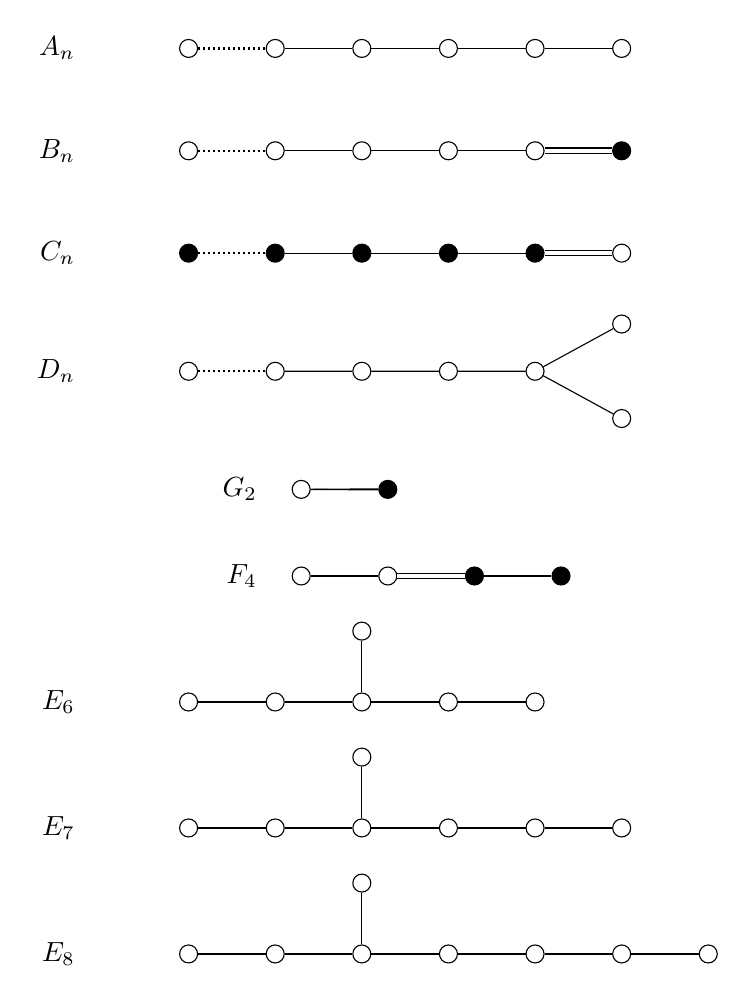
\begin{tikzpicture}[x=1.1cm,y=1cm,
  wv/.style={circle,draw,fill=white,inner sep=0pt,minimum size=6.5pt},
  bv/.style={circle,draw,fill=black,inner sep=0pt,minimum size=6.5pt},
  lab/.style={anchor=east}]
% A_n
\node[lab] at (-1.2,0) {$A_{n}$};
\foreach \i in {0,...,5} \node[wv] (A\i) at (\i,0) {};
\draw[densely dotted,thick] (A0)--(A1);
\draw (A1)--(A2) (A2)--(A3) (A3)--(A4) (A4)--(A5);
% B_n
\node[lab] at (-1.2,-1.3) {$B_{n}$};
\foreach \i in {0,...,4} \node[wv] (B\i) at (\i,-1.3) {};
\node[bv] (B5) at (5,-1.3) {};
\draw[densely dotted,thick] (B0)--(B1);
\draw (B1)--(B2) (B2)--(B3) (B3)--(B4);
\draw[double,double distance=1.6pt] (B4)--(B5);
% C_n
\node[lab] at (-1.2,-2.6) {$C_{n}$};
\foreach \i in {0,...,4} \node[bv] (C\i) at (\i,-2.6) {};
\node[wv] (C5) at (5,-2.6) {};
\draw[densely dotted,thick] (C0)--(C1);
\draw (C1)--(C2) (C2)--(C3) (C3)--(C4);
\draw[double,double distance=1.6pt] (C4)--(C5);
% D_n
\node[lab] at (-1.2,-4.1) {$D_{n}$};
\foreach \i in {0,...,4} \node[wv] (D\i) at (\i,-4.1) {};
\node[wv] (D5) at (5,-3.5) {};
\node[wv] (D6) at (5,-4.7) {};
\draw[densely dotted,thick] (D0)--(D1);
\draw (D1)--(D2) (D2)--(D3) (D3)--(D4) (D4)--(D5) (D4)--(D6);
% G_2
\node[lab] at (0.9,-5.6) {$G_{2}$};
\node[wv] (G0) at (1.3,-5.6) {};
\node[bv] (G1) at (2.3,-5.6) {};
\draw (G0)--(G1);
\draw ([yshift=1.7pt]G0)--([yshift=1.7pt]G1);
\draw ([yshift=-1.7pt]G0)--([yshift=-1.7pt]G1);
% F_4
\node[lab] at (0.9,-6.7) {$F_{4}$};
\node[wv] (F0) at (1.3,-6.7) {};
\node[wv] (F1) at (2.3,-6.7) {};
\node[bv] (F2) at (3.3,-6.7) {};
\node[bv] (F3) at (4.3,-6.7) {};
\draw (F0)--(F1);
\draw[double,double distance=1.6pt] (F1)--(F2);
\draw (F2)--(F3);
% E_6
\node[lab] at (-1.2,-8.3) {$E_{6}$};
\foreach \i in {0,...,4} \node[wv] (E6\i) at (\i,-8.3) {};
\node[wv] (E6t) at (2,-7.4) {};
\draw (E60)--(E61) (E61)--(E62) (E62)--(E63) (E63)--(E64) (E62)--(E6t);
% E_7
\node[lab] at (-1.2,-9.9) {$E_{7}$};
\foreach \i in {0,...,5} \node[wv] (E7\i) at (\i,-9.9) {};
\node[wv] (E7t) at (2,-9.0) {};
\draw (E70)--(E71) (E71)--(E72) (E72)--(E73) (E73)--(E74) (E74)--(E75) (E72)--(E7t);
% E_8
\node[lab] at (-1.2,-11.5) {$E_{8}$};
\foreach \i in {0,...,6} \node[wv] (E8\i) at (\i,-11.5) {};
\node[wv] (E8t) at (2,-10.6) {};
\draw (E80)--(E81) (E81)--(E82) (E82)--(E83) (E83)--(E84) (E84)--(E85) (E85)--(E86) (E82)--(E8t);
\end{tikzpicture}
\end{center}
反之，这些图中的每一个都是某个``不可约''的既约根系的 Dynkin 图.
\end{theorem*}
这两个分类定理告诉我们，单 Lie 代数由上面的 Dynkin 图分类. 至于经典 Lie 代数，通过计算可以验证 $\mathfrak{sl}_{n}\leftrightarrow A_{n-1}$、$\mathfrak{so}_{2n+1}\leftrightarrow B_{n}$、$\mathfrak{sp}_{2n}\leftrightarrow C_{n}$ 以及 $\mathfrak{so}_{2n}\leftrightarrow D_{n}$（$n\geqslant 3$）. 其余的单 Lie 代数（其数目有限）称为``例外''的.
\end{numpara}
